\documentclass[11pt]{article}\usepackage[]{graphicx}\usepackage[]{color}
%% maxwidth is the original width if it is less than linewidth
%% otherwise use linewidth (to make sure the graphics do not exceed the margin)
\makeatletter
\def\maxwidth{ %
  \ifdim\Gin@nat@width>\linewidth
    \linewidth
  \else
    \Gin@nat@width
  \fi
}
\makeatother

\definecolor{fgcolor}{rgb}{0.345, 0.345, 0.345}
\newcommand{\hlnum}[1]{\textcolor[rgb]{0.686,0.059,0.569}{#1}}%
\newcommand{\hlstr}[1]{\textcolor[rgb]{0.192,0.494,0.8}{#1}}%
\newcommand{\hlcom}[1]{\textcolor[rgb]{0.678,0.584,0.686}{\textit{#1}}}%
\newcommand{\hlopt}[1]{\textcolor[rgb]{0,0,0}{#1}}%
\newcommand{\hlstd}[1]{\textcolor[rgb]{0.345,0.345,0.345}{#1}}%
\newcommand{\hlkwa}[1]{\textcolor[rgb]{0.161,0.373,0.58}{\textbf{#1}}}%
\newcommand{\hlkwb}[1]{\textcolor[rgb]{0.69,0.353,0.396}{#1}}%
\newcommand{\hlkwc}[1]{\textcolor[rgb]{0.333,0.667,0.333}{#1}}%
\newcommand{\hlkwd}[1]{\textcolor[rgb]{0.737,0.353,0.396}{\textbf{#1}}}%

\usepackage{framed}
\makeatletter
\newenvironment{kframe}{%
 \def\at@end@of@kframe{}%
 \ifinner\ifhmode%
  \def\at@end@of@kframe{\end{minipage}}%
  \begin{minipage}{\columnwidth}%
 \fi\fi%
 \def\FrameCommand##1{\hskip\@totalleftmargin \hskip-\fboxsep
 \colorbox{shadecolor}{##1}\hskip-\fboxsep
     % There is no \\@totalrightmargin, so:
     \hskip-\linewidth \hskip-\@totalleftmargin \hskip\columnwidth}%
 \MakeFramed {\advance\hsize-\width
   \@totalleftmargin\z@ \linewidth\hsize
   \@setminipage}}%
 {\par\unskip\endMakeFramed%
 \at@end@of@kframe}
\makeatother

\definecolor{shadecolor}{rgb}{.97, .97, .97}
\definecolor{messagecolor}{rgb}{0, 0, 0}
\definecolor{warningcolor}{rgb}{1, 0, 1}
\definecolor{errorcolor}{rgb}{1, 0, 0}
\newenvironment{knitrout}{}{} % an empty environment to be redefined in TeX

\usepackage{alltt}

% margins, size, formatting
\oddsidemargin=0in
\evensidemargin=0in
\topmargin=0in
\textwidth=6.5in
\textheight=9.5in
\parindent = 0 in
\pagestyle{plain}

    \usepackage[
    bottom = 2.50cm]{geometry}

\usepackage{amsmath,amssymb,amsthm, amsfonts}
\usepackage{array}
\usepackage{fancyhdr}
%\pagestyle{plain}
\pagestyle{fancy}
%\usepackage{listings}
%\usepackage{inconsolata}

\lhead{\textbf{Group 3: Model Selection}}
\rhead{\textbf{Emily Ramos}}
\cfoot{}
\IfFileExists{upquote.sty}{\usepackage{upquote}}{}

\begin{document}




\section{Initial Model}

As stated previously, the initial model we are interested in fitting is of the form:\\
weight$_i = \beta_0 + \beta_1$ chest.diam$_{i} + \beta_2$ chest.dep$_{i} + \beta_3$ bitro.diam$_{i} + \beta_4$ wrist.min$_{i} + \beta_5$ ankle.min$_{i} + \beta_6$ height$_{i}$




\begin{knitrout}
\definecolor{shadecolor}{rgb}{0.969, 0.969, 0.969}\color{fgcolor}\begin{kframe}
\begin{verbatim}
## (Intercept)  chest.diam   chest.dep  bitro.diam   wrist.min 
##    -109.890       1.340       1.537       1.196       1.113 
##   ankle.min      height 
##       1.152       0.177
\end{verbatim}
\end{kframe}
\end{knitrout}


This model indicates that the expected change in weight for a 1 unit change in chest.diam, holding all other variables constant, is 1.34 lbs. The expected change in weight for a 1 unit change in chest.dep, holding all other variables constant, is 1.54 lbs., etc. Note that chest depth has the largest impact on weight. In addition to the coefficients, the R-squared value of 0.8882 implies that our model explains 88.82\% of the variation in weight and the $P$-values for each variable and for the model are significant. This model seems like a good tool to predict weight given these measurements, but are there better ones?

\section{Model Selection}

We are building a model to predict weight given various body measurements. Before running random models, we need to determine what predictors to use. The predictors needed in our models are age, height and gender. These variables contribute significantly to weight. The predictors we will allow in model selection are the initial predictors: chest diameter, chest depth and bitro diameter. In addition to these variables, pelvic bredth, shoulder, chest, waist, hip and thigh will be used. I chose to allow these predictors in my model since these are directly associated with weight (e.g. waist). However, for the other models we will fit, we will let ``R" do it's work.

\subsection{Criterion}

The Information Criterions we will be using to evaluate our models are Akaike Information Crierion (AIC), Bayes Information Criterion (BIC), adjusted $R^2$ and Predictive Residual Sum of Squares (PReSS). In short, AIC and BIC measure goodness-of-fit through residual sum of squares (log likelihoods) and penalizes the model size; the smaller the AIC/BIC, the better. Adjusted $R^2$ adjusts $R^2$ so that the model is penalized for adding more predictors; the higher the value of the adjusted $R^2$ the better. Finally, PRESS is a summary measure focused on prediction; the lower the value of PRESS, the better.
\begin{eqnarray*}
\text{AIC} &=& n\log \left(\dfrac{RSS}{n}\right) + 2(p +1)\\
\text{BIC} &=& n\log \left(\dfrac{RSS}{n}\right) + (p + 1) \log(n)\\
\text{adj}R^2 &=& 1 - \dfrac{n - 1}{n - p - 1}(1 - R^2)\\
\end{eqnarray*}
\begin{eqnarray*}
\text{PRESS} &=& \sum{\left(\dfrac{\hat{\epsilon}_i}{1 - h_{ii}}\right)^2}
\end{eqnarray*}

\subsection{Methods in R}

There are multiple methods built into different packages in R for Model Selection. To illustrate these, we will use the variables:  height, wrist.min, ankle.min and chest and call this model ``MLRex".



\subsubsection{stepAIC()}\\
The R function found in the package ``MASS" called ``stepAIC()" performs stepwise model selection by AIC. This will output the initial model and the final model (model of best fit determined by this method), and the steps taken. In the output below we can see that this method suggests using a different model that doesn't contain wrist.diam.\\




\texttt{Initial Model: weight ~ height + wrist.diam + ankle.diam + chest\\
Final Model: weight ~ height + ankle.diam + chest\\
\begin{tabular}{r r r r r r r}
        &  Step & Df & Deviance & Resid. Df & Resid. Dev & AIC \\
1  &            &      &        &  502 &  13294.14 & 1666.150 \\
2 & - wrist.diam & 1 & 47.90427 & 503 &   13342.05 & 1665.974
\end{tabular}
}

\subsubsection{leaps()}\\
The R package ``leaps" contains a function ``regsubsets()". This method performs an exhaustive search of models and plots the $R^2$ criterion by variables and subset size. The class ``summary.regsubsets" outputs an object with multiple elements, including adjusted $R^2$ and BIC. Furthermore, the plots below plot the  
BIC and Adjusted $R^2$ values against each subset of variables. 

\begin{knitrout}
\definecolor{shadecolor}{rgb}{0.969, 0.969, 0.969}\color{fgcolor}
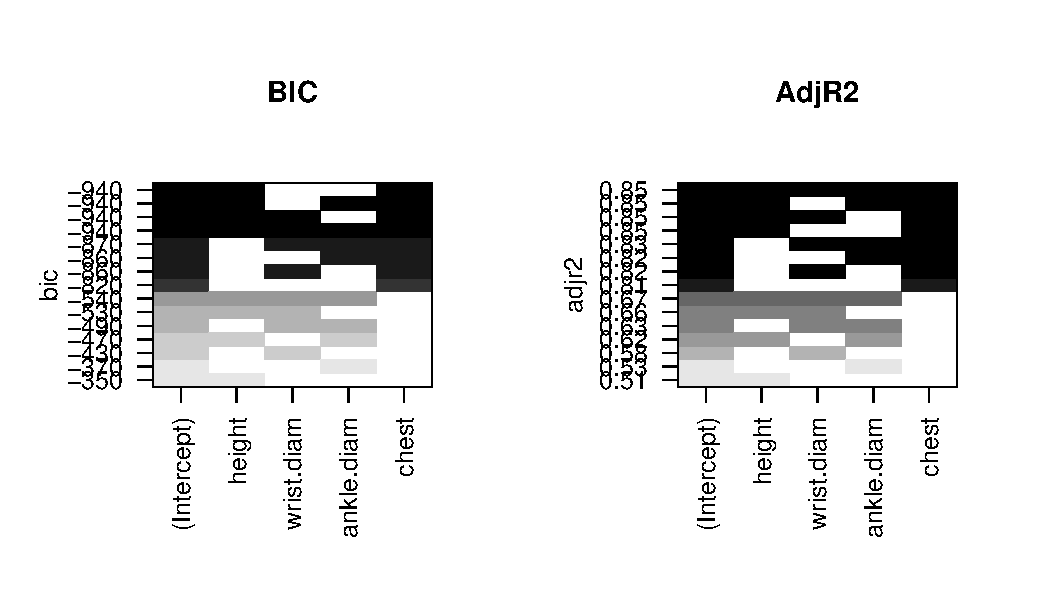
\includegraphics[width=\maxwidth]{figure/leap} 

\end{knitrout}


In these plots, for example, the BIC plot is implying the best model is using height and chest as predictors. On the other hand, the AdjR2 plot is saying all variables give the best fit. Using both of these plots together, one might conflude height, ankle.diam and chest would be the best fit. This conclsion agrees with our analysis using stepAIC.

\subsection{Model Selection in Action}




The Model Selection Lab will explain how to obtain the models summarized in Table 1.     

\textbf{Table 1}\\

\begin{center}
\begin{tabular}{|r|c|c|c|c|r|}
  \hline
MLR\# & AIC & BIC & PRESS & Adjusted $R^2$ & Method \\ 
  \hline
all & 2216 & 2324 & 2383 & 0.9753 & \text{all variables  from dataset used} \\ \hline
i & 2970 & 3004 & 10405 & 0.8869 & \text{suggested by paper} \\ \hline
1 & 2256 & 2319 & 2560 & 0.9727 & \text{suggested by paper}\\ \hline
2 & 2402 & 2441 & 3408 & 0.9632 & \text{my model}\\ \hline
3 & 2206 & 2282 & 2329 & 0.9754 & \text{stepAIC} \\ \hline
4 & 2195 & 2271 & 2281 & 0.9759 & \text{stepAIC and adjustments} \\ \hline
5 & 2207 & 2292 & 2335 & 0.9755 &\text{leaps (adj} R^2) \\ \hline
6 & 2189 & 2278 & 2255 & \textcolor{0.9764}  & \text{leaps(adj} R^2) \text{and adjustments}\\ \hline
7 & 2213 & 2272 & 2353 & 0.9749 & \text{leaps(BIC)} \\ \hline
8 & \textcolor{red}{2194} & \textcolor{red}{2257} & \textcolor{red}{2267} & 0.9759 & \text{leaps(BIC) and adjustments}\\ \hline
\end{tabular}
\end{center}

Base on Table 1, we can see that each Criterion yields different results. It is up to our discretion to choose a model. Since AIC and BIC are lowest in MLR8, the adjusted $R^2$ is the larges, and the PRESS is close to 2300, I would choose MLR8 as the model of best fit. MLR8 is of the form:\\ 
weight$_i = \beta_0 + \beta_1$ chest.dep$_{i} + \beta_2$ knee.diam$_{i} + \beta_3$ shoulder$_{i} + \beta_4$ chest$_{i}$ + \beta_5$ waist$_{i} + \beta_6$ hip$_{i}$ + 
\beta_7$ thigh$_{i}$ + \beta_7$ forearm$_{i}$ + \beta_8$ calf$_{i}$ + \beta_9$ gender$_{i}$ + \beta_{10}$ height$_{i}$ + \beta_{11}$ height$^2_{i} + \beta_{12}$ age$^2_{i}$.

\begin{knitrout}
\definecolor{shadecolor}{rgb}{0.969, 0.969, 0.969}\color{fgcolor}\begin{kframe}
\begin{verbatim}
## (Intercept)   chest.dep   knee.diam    shoulder       chest 
##  -1.512e+01   2.268e-01   6.364e-01   8.838e-02   1.673e-01 
##       waist         hip       thigh     forearm        calf 
##   3.779e-01   2.454e-01   2.469e-01   5.989e-01   4.210e-01 
##      height      gender    I(age^2) I(height^2) 
##  -9.414e-01  -1.480e+00  -7.361e-04   3.667e-03
\end{verbatim}
\end{kframe}
\end{knitrout}


\section{Conclusion}
Model Selection truely is an art form. R can mechanically run through steps, interactions, combinations, etc. However, R cannot subjectively look at the variables to determine the absolute best model. To acheive the model of best fit, a combination of methods and human adjustment is necessary.

\end{document}
